% ============================================================
%  D-HNSW: Deterministic Hierarchical Navigable Small World
%  Graphs for Verifiable Nearest Neighbor Search
%  IEEE Transactions on Knowledge and Data Engineering
% ============================================================
\documentclass[10pt,journal,compsoc]{IEEEtran}

% ---- Packages ----
\usepackage[utf8]{inputenc}
\usepackage[T1]{fontenc}
\usepackage{amsmath,amssymb,amsfonts}
\usepackage{algorithmic}
\usepackage{algorithm}
\usepackage{graphicx}
\usepackage{textcomp}
\usepackage{xcolor}
\usepackage{booktabs}
\usepackage{multirow}
\usepackage{hyperref}
\usepackage{cleveref}
\usepackage{balance}
\usepackage{subcaption}
\usepackage{enumitem}
\usepackage{url}
\usepackage{cite}

% ---- Custom commands ----
\newcommand{\dhnsw}{\textsc{D-HNSW}}
\newcommand{\hnsw}{\textsc{HNSW}}
\newcommand{\ie}{\textit{i.e.}}
\newcommand{\eg}{\textit{e.g.}}
\newcommand{\etal}{\textit{et~al.}}
\newcommand{\wrt}{w.r.t.}
\newcommand{\recall}{\text{Recall@10}}

\hypersetup{
  colorlinks=true,
  linkcolor=blue!70!black,
  citecolor=green!50!black,
  urlcolor=blue!70!black
}

\begin{document}

% ---- Title ----
\title{D-HNSW: Deterministic Hierarchical Navigable Small World Graphs\\for Verifiable Nearest Neighbor Search}

\author{
  \IEEEauthorblockN{Anonymous Authors}
  \IEEEauthorblockA{Under Review}
}

\IEEEtitleabstractindextext{%

% ---- Abstract ----
\begin{abstract}
Approximate nearest neighbor (ANN) search is a cornerstone of modern data-intensive applications, from recommendation systems to retrieval-augmented generation. The Hierarchical Navigable Small World (HNSW) algorithm has emerged as the dominant index structure due to its superior recall-throughput tradeoff. However, HNSW relies on IEEE~754 floating-point arithmetic, which introduces platform-dependent nondeterminism through variations in instruction reordering, fused multiply-add availability, and SIMD lane widths. This nondeterminism renders search results unverifiable---a critical limitation for blockchain-based systems, decentralized AI, and regulatory-compliant deployments where independent parties must reproduce identical results.

We present \dhnsw{} (Deterministic HNSW), a modified HNSW algorithm that guarantees bit-exact reproducibility across all platforms by replacing floating-point distance computations with 64-bit fixed-point integer arithmetic. Our fixed-point representation uses a Q32.32 format with saturating operations and achieves distance computation errors below $10^{-8}$ relative to IEEE~754 double precision. To mitigate the inherent performance overhead of integer arithmetic, we introduce a suite of optimizations including SIMD-accelerated fixed-point operations, two-phase distance computation with early termination, and partial distance pruning.

Extensive experiments on six benchmark datasets (SIFT-128, GloVe-100, Fashion-MNIST-784, GIST-960, Deep-96, and Random-128) demonstrate that \dhnsw{} achieves \textbf{identical} recall to standard HNSW while maintaining 57.1\% of its throughput at the operating point of $\text{ef}=128$ on SIFT-1M. Ablation studies show that our optimization pipeline reduces the na\"ive fixed-point overhead from $2.10\times$ to $1.75\times$. Determinism is verified through SHA-256 hash comparison across five independent executions, confirming bit-exact result reproducibility with zero hash collisions. The system scales to one million vectors while maintaining consistent overhead ratios, demonstrating practical viability for production deployment in trust-critical environments.
\end{abstract}

% ---- Keywords ----
\begin{IEEEkeywords}
Approximate nearest neighbor search, deterministic computation, fixed-point arithmetic, HNSW, blockchain, verifiable AI, vector databases
\end{IEEEkeywords}
}

\maketitle

% ============================================================
%  I. INTRODUCTION
% ============================================================
\section{Introduction}
\IEEEPARstart{A}{pproximate} nearest neighbor (ANN) search has become an indispensable primitive in modern computing, underpinning applications from large-scale information retrieval~\cite{jegou2011pq} and recommendation systems to the retrieval-augmented generation (RAG) pipelines that power contemporary large language models. As vector databases grow to billions of entries~\cite{simhadri2022neurips}, the demand for algorithms that balance search quality (recall) with computational efficiency (throughput) has intensified. Among the diverse family of ANN algorithms---including tree-based methods~\cite{bentley1975kdtree}, locality-sensitive hashing~\cite{gionis1999lsh}, product quantization~\cite{jegou2011pq}, and graph-based approaches~\cite{malkov2014nsw}---the Hierarchical Navigable Small World (\hnsw{}) algorithm~\cite{malkov2020hnsw} has established itself as the de facto standard, consistently achieving state-of-the-art recall-throughput tradeoffs across major benchmarks~\cite{simhadri2022neurips} and serving as the backbone of production systems such as Faiss~\cite{douze2024faiss}, Qdrant, Weaviate, and Milvus.

Despite its effectiveness, \hnsw{} harbors a fundamental limitation that has received insufficient attention: \emph{nondeterminism}. Standard \hnsw{} implementations rely on IEEE~754 floating-point arithmetic for distance computations, which, while providing excellent numerical range and precision, does not guarantee identical results across different hardware platforms, compiler optimization levels, or instruction set architectures~\cite{goldberg1991float}. Floating-point nondeterminism arises from multiple sources: (1)~the availability and use of fused multiply-add (FMA) instructions, which compute $a \times b + c$ with a single rounding step rather than two; (2)~compiler-driven instruction reordering that exploits algebraic properties not preserved under finite-precision arithmetic; (3)~variations in SIMD lane widths (SSE, AVX2, AVX-512, NEON) that change the order of partial-sum accumulation; and (4)~transcendental function implementations that differ across math libraries. These seemingly minor discrepancies can propagate through the greedy graph traversal of \hnsw{}, where a single tie-breaking difference in distance comparison may redirect the search path, potentially yielding entirely different result sets.

For many traditional applications, such nondeterminism is inconsequential---a search engine returning slightly different results across servers is perfectly acceptable. However, a growing class of applications \emph{requires} deterministic, verifiable computation:

\begin{itemize}[leftmargin=*]
  \item \textbf{Blockchain and smart contracts.} Decentralized systems require all validator nodes to reach identical state transitions from identical inputs~\cite{buterin2014ethereum, lai2022blockchain}. A vector similarity search embedded in a smart contract must produce bit-exact results regardless of the validator's hardware, or consensus will fail. Cardano's EUTXO model explicitly mandates deterministic transaction evaluation~\cite{cardano2024fees}, and integer arithmetic is widely recognized as essential for blockchain consensus~\cite{decenomy2024integer}.

  \item \textbf{Verifiable and auditable AI.} As AI systems are deployed in regulated domains---healthcare diagnostics, financial credit scoring, autonomous vehicles---regulators increasingly demand that inference results be reproducible and auditable~\cite{alves2026eigenai}. Floating-point nondeterminism undermines this requirement, as demonstrated by recent work on nondeterminism-aware verification~\cite{yao2025nao}.

  \item \textbf{Decentralized vector databases.} Emerging Web3 architectures for similarity search~\cite{keizer2023ditto, lee2024decentface} and AI-powered data trading~\cite{zhang2024nmft} require that query results be independently verifiable. ANNProof~\cite{lu2024annproof} addresses verification at the proof level but does not eliminate the underlying nondeterminism in distance computation.

  \item \textbf{Deterministic AI infrastructure.} Projects such as Valori~\cite{gudur2025valori} and EigenAI~\cite{alves2026eigenai} are building deterministic substrates for AI computation, recognizing that reproducibility is a prerequisite for trust in distributed AI systems.
\end{itemize}

\noindent\textbf{Our contribution.} We present \dhnsw{}, a deterministic variant of the \hnsw{} algorithm that guarantees bit-exact reproducibility across all platforms. The key insight is to replace IEEE~754 floating-point distance computations with 64-bit fixed-point integer arithmetic, which produces identical results on any hardware that supports standard integer operations---effectively all modern processors. Our specific contributions are:

\begin{enumerate}[leftmargin=*]
  \item \textbf{Fixed-point distance computation framework.} We design a Q32.32 fixed-point arithmetic system with saturating operations, supporting squared Euclidean distance, Euclidean distance (via Newton--Raphson integer square root), and cosine similarity. We provide formal error bounds showing relative errors below $10^{-8}$ compared to IEEE~754 double precision (\Cref{sec:method}).

  \item \textbf{Performance optimization suite.} We introduce five complementary optimizations---SIMD-accelerated fixed-point operations, two-phase distance computation, neighbor reordering, early termination, and partial distance pruning---that collectively reduce the na\"ive fixed-point overhead from $2.10\times$ to $1.75\times$ (\Cref{sec:optimizations}).

  \item \textbf{Deterministic graph construction.} We replace all sources of nondeterminism in the \hnsw{} index construction process, including the random level generator, with a deterministic alternative based on a seeded Keccak-256 permutation~\cite{bertoni2013keccak}, ensuring that both index building and querying are fully reproducible (\Cref{sec:construction}).

  \item \textbf{Comprehensive empirical evaluation.} We evaluate \dhnsw{} on six diverse benchmark datasets spanning 96 to 960 dimensions, demonstrating identical recall, verified determinism through SHA-256 hashing, and practical throughput of 57.1\% of standard \hnsw{} across all datasets (\Cref{sec:experiments}).
\end{enumerate}

The remainder of this paper is organized as follows. \Cref{sec:related} surveys related work on ANN search, deterministic computation, and blockchain applications. \Cref{sec:background} provides necessary background on \hnsw{} and floating-point nondeterminism. \Cref{sec:method} presents the \dhnsw{} fixed-point arithmetic framework. \Cref{sec:optimizations} details our performance optimizations. \Cref{sec:construction} describes deterministic graph construction. \Cref{sec:experiments} presents experimental results. \Cref{sec:discussion} discusses implications and limitations, and \Cref{sec:conclusion} concludes.


% ============================================================
%  II. RELATED WORK
% ============================================================
\section{Related Work}
\label{sec:related}

\subsection{Approximate Nearest Neighbor Search}

The ANN problem has been studied extensively across multiple algorithmic paradigms. \textbf{Tree-based methods}, originating with KD-trees~\cite{bentley1975kdtree}, partition the space hierarchically but suffer from the curse of dimensionality, degrading to linear scan beyond approximately 20 dimensions. \textbf{Hashing-based methods}, notably locality-sensitive hashing (LSH)~\cite{gionis1999lsh}, provide sublinear query time with theoretical guarantees but require substantial memory overhead for high recall. \textbf{Quantization-based methods}, particularly product quantization (PQ)~\cite{jegou2011pq} and its variants~\cite{baranchuk2018revisiting}, achieve excellent compression ratios but introduce quantization error that limits recall at high precision operating points.

\textbf{Graph-based methods} have emerged as the dominant paradigm for high-recall ANN search. The Navigable Small World (NSW) algorithm~\cite{malkov2014nsw} constructs a proximity graph with long-range links that enable logarithmic-time greedy routing. \hnsw{}~\cite{malkov2020hnsw} extends NSW with a hierarchical structure inspired by skip lists, where upper layers contain progressively sparser subsets of nodes, enabling coarse-to-fine navigation. This design achieves $O(\log n)$ expected search complexity while maintaining high recall, and has been validated at billion scale~\cite{simhadri2022neurips}. DiskANN~\cite{subramanya2019diskann} adapts graph-based search for disk-resident indices, while BANG~\cite{karthik2024bang} leverages GPU parallelism. HARMONY~\cite{xu2025harmony} addresses distributed deployment. Recent work by Teofili and Lin~\cite{teofili2025patience} introduces patience-based early termination for \hnsw{} traversal, a strategy complementary to our approach.

Despite the maturity of ANN algorithms, none of the above works address the determinism of distance computation. All assume IEEE~754 floating-point arithmetic and implicitly accept platform-dependent variation in results.

\subsection{Deterministic Computation and Blockchain}

The requirement for deterministic execution is well-established in blockchain systems. Ethereum~\cite{buterin2014ethereum} achieves consensus by requiring all nodes to execute identical EVM bytecode and arrive at the same state. Cardano's EUTXO model goes further by mandating deterministic transaction evaluation, where transaction fees and outcomes are predictable before submission~\cite{cardano2024fees}. The Decenomy project~\cite{decenomy2024integer} explicitly identifies integer arithmetic as essential for blockchain consensus, noting that floating-point operations can produce different results across validator nodes.

Lai~\etal{}~\cite{lai2022blockchain} study the intersection of private blockchains and deterministic databases, demonstrating that database operations must be carefully constrained to maintain consensus. Olivieri~\etal{}~\cite{olivieri2022golisa} present GoLiSA, a static analysis tool for ensuring determinism in blockchain software, highlighting the practical difficulty of eliminating nondeterministic behavior from complex software systems.

In the AI domain, Yao~\etal{}~\cite{yao2025nao} address nondeterminism in floating-point neural network verification, proposing optimistic verification strategies that account for platform-dependent variation. EigenAI~\cite{alves2026eigenai} and Valori~\cite{gudur2025valori} represent emerging efforts to build deterministic AI infrastructure, recognizing that verifiable computation requires eliminating all sources of nondeterminism, including floating-point arithmetic.

\subsection{Vector Search on Blockchain}

Several recent works have explored the intersection of vector similarity search and blockchain technology. ANNProof~\cite{lu2024annproof} builds a verifiable outsourced ANN search system on blockchain, using cryptographic proofs to verify that search results are correct. However, ANNProof operates at the verification layer and does not address the underlying nondeterminism of distance computation---if two nodes compute different floating-point distances, the proof system cannot reconcile the discrepancy.

Keizer~\etal{}~\cite{keizer2023ditto} propose Ditto, a decentralized similarity search system for Web3 services that distributes the index across multiple nodes. Lee and Chen~\cite{lee2024decentface} implement decentralized face identification using \hnsw{} on blockchain. Zhang~\cite{zhang2024nmft} introduces NMFT, a data trading protocol that combines NFTs with AI-powered Merkle feature trees for copyright verification. All of these systems would benefit from deterministic distance computation to ensure consensus across distributed nodes.

\textbf{Positioning of \dhnsw{}.} Our work is complementary to and distinct from the above efforts. While ANNProof provides verification \emph{after} computation, \dhnsw{} ensures determinism \emph{during} computation. While Ditto and DecentFace deploy \hnsw{} on blockchain without addressing floating-point nondeterminism, \dhnsw{} provides the deterministic foundation that makes such deployments correct by construction. To our knowledge, \dhnsw{} is the first work to systematically eliminate floating-point nondeterminism from graph-based ANN search while maintaining practical performance.

% ============================================================
%  III. BACKGROUND
% ============================================================
\section{Background}
\label{sec:background}

\subsection{HNSW Algorithm}

The \hnsw{} algorithm~\cite{malkov2020hnsw} constructs a multi-layer proximity graph where each layer $\ell \in \{0, 1, \ldots, L\}$ contains a subset of the dataset vectors. Layer~0 contains all $n$ vectors, while higher layers contain exponentially fewer nodes, with the probability of a vector appearing at layer $\ell$ given by $p(\ell) = e^{-\ell / m_L}$, where $m_L$ is a normalization factor.

\textbf{Index construction.} Each vector $v$ is inserted by first determining its maximum layer $\ell_v$ via random sampling. Starting from the entry point at the top layer, a greedy search descends through layers $L, L{-}1, \ldots, \ell_v{+}1$, finding the nearest neighbor at each layer. From layer $\ell_v$ down to layer~0, the algorithm performs a beam search with width \texttt{efConstruction} to identify the $M$ nearest neighbors, which become the edges of $v$ in the graph. A heuristic pruning step ensures that edges are diverse, preferring neighbors that are not too close to each other.

\textbf{Search.} Given a query $q$, the search begins at the entry point on the top layer and greedily descends to layer~1. At layer~0, a beam search with width \texttt{ef} (the search parameter) explores the graph, maintaining a priority queue of candidates and a result set of the \texttt{ef} nearest vectors found so far. The search terminates when no candidate in the queue is closer to $q$ than the farthest element in the result set. The top-$k$ results are extracted from the final result set.

\textbf{Distance computation.} The core operation in both construction and search is distance computation between vectors. For $d$-dimensional vectors $\mathbf{x}, \mathbf{y} \in \mathbb{R}^d$, the squared Euclidean distance is:
\begin{equation}
  \label{eq:l2dist}
  D(\mathbf{x}, \mathbf{y}) = \sum_{i=1}^{d} (x_i - y_i)^2
\end{equation}
This computation dominates the runtime of \hnsw{}, accounting for over 90\% of total execution time in typical workloads.

\subsection{Floating-Point Nondeterminism}
\label{sec:fp_nondet}

IEEE~754 floating-point arithmetic~\cite{goldberg1991float} is nondeterministic across platforms for several reasons:

\textbf{Fused multiply-add (FMA).} The FMA instruction computes $a \times b + c$ with a single rounding, while the separate multiply-then-add sequence rounds twice. The difference is at most one unit in the last place (ULP), but this suffices to change comparison outcomes. FMA availability varies: x86 processors gained FMA3 with Haswell (2013), while ARM NEON has always included it.

\textbf{Instruction reordering.} Compilers may reorder floating-point additions to improve instruction-level parallelism. Since floating-point addition is not associative---$(a + b) + c \neq a + (b + c)$ in general---different summation orders produce different results. The accumulation order in \Cref{eq:l2dist} is particularly sensitive, as it involves $d$ additions of squared differences.

\textbf{SIMD vectorization.} Different SIMD widths (128-bit SSE, 256-bit AVX2, 512-bit AVX-512) process different numbers of elements per instruction, leading to different partial-sum trees and thus different final results. A distance computation using AVX-512 (8 floats per lane) will generally differ from one using SSE (4 floats per lane).

\textbf{Propagation through graph traversal.} In \hnsw{}, a distance difference of even one ULP can change the ordering of candidates in the priority queue. Since the greedy search follows the nearest candidate at each step, a single reordering can redirect the entire search path, potentially visiting completely different regions of the graph and returning different result sets. This amplification effect means that platform-dependent floating-point variation is not merely a numerical nuisance but a correctness concern for applications requiring deterministic results.

\subsection{Fixed-Point Arithmetic}

Fixed-point arithmetic represents real numbers as scaled integers, with a fixed number of bits allocated to the integer and fractional parts. A Q$m$.$f$ format uses $m$ bits for the integer part and $f$ bits for the fractional part, representing values in the range $[-2^{m-1}, 2^{m-1} - 2^{-f}]$ with resolution $2^{-f}$.

The key advantage of fixed-point arithmetic for determinism is that all operations reduce to integer arithmetic (addition, subtraction, multiplication, and bit shifts), which is defined to produce identical results on all platforms conforming to the C/Rust language standards. There is no platform-dependent rounding mode, no FMA ambiguity, and no SIMD-width-dependent accumulation order (when the summation order is fixed in software).

The primary disadvantage is reduced dynamic range compared to floating-point. A 64-bit fixed-point Q32.32 format provides approximately $9.6$ decimal digits of precision with a range of $\pm 2^{31} \approx \pm 2.1 \times 10^9$, compared to IEEE~754 double precision's approximately $15.9$ decimal digits with a range of $\pm 1.8 \times 10^{308}$. For ANN search, where vector components are typically normalized or bounded, this range is sufficient, as we demonstrate empirically.


% ============================================================
%  IV. D-HNSW: FIXED-POINT DISTANCE COMPUTATION
% ============================================================
\section{D-HNSW: Fixed-Point Distance Framework}
\label{sec:method}

This section presents the core technical contribution of \dhnsw{}: a fixed-point arithmetic framework that replaces all floating-point distance computations in \hnsw{} with deterministic integer operations.

\subsection{Q32.32 Fixed-Point Representation}

We adopt a Q32.32 fixed-point format, where each value is stored as a 64-bit signed integer with 32 bits for the integer part and 32 bits for the fractional part. The mapping between a real value $r$ and its fixed-point representation $\hat{r}$ is:
\begin{equation}
  \label{eq:fp_encode}
  \hat{r} = \lfloor r \times 2^{32} + 0.5 \rfloor
\end{equation}
and the inverse mapping is $r \approx \hat{r} / 2^{32}$. The representation error from quantization is bounded by:
\begin{equation}
  |r - \hat{r}/2^{32}| \leq 2^{-33} \approx 1.16 \times 10^{-10}
\end{equation}

\textbf{Saturating operations.} To prevent integer overflow from silently corrupting results, we implement all arithmetic operations with saturation semantics:
\begin{align}
  \text{sat\_add}(a, b) &= \text{clamp}(a + b, -2^{63}, 2^{63}{-}1) \\
  \text{sat\_sub}(a, b) &= \text{clamp}(a - b, -2^{63}, 2^{63}{-}1) \\
  \text{sat\_mul}(a, b) &= \text{clamp}((a \times b) \gg 32, -2^{63}, 2^{63}{-}1)
\end{align}
where $\gg$ denotes arithmetic right shift. The multiplication uses 128-bit intermediate results (available on all 64-bit platforms) to avoid precision loss before the shift.

\subsection{Vector Representation}

Each $d$-dimensional vector $\mathbf{x} = (x_1, \ldots, x_d)$ is converted to a fixed-point vector $\hat{\mathbf{x}} = (\hat{x}_1, \ldots, \hat{x}_d)$ using \Cref{eq:fp_encode}. The conversion is performed once during index construction and stored persistently. The \texttt{FixedPointVector<D>} structure in our Rust implementation stores the $d$ components as an array of \texttt{i64} values with compile-time dimension checking via const generics.

\subsection{Distance Metrics}

\textbf{Squared Euclidean distance.} The squared $L_2$ distance between fixed-point vectors $\hat{\mathbf{x}}$ and $\hat{\mathbf{y}}$ is computed as:
\begin{equation}
  \label{eq:fp_l2}
  \hat{D}(\hat{\mathbf{x}}, \hat{\mathbf{y}}) = \sum_{i=1}^{d} \text{sat\_mul}(\hat{x}_i - \hat{y}_i,\; \hat{x}_i - \hat{y}_i)
\end{equation}
where the subtraction and accumulation use saturating operations. The summation order is fixed (index 1 through $d$), eliminating the associativity-dependent variation of floating-point accumulation.

\textbf{Euclidean distance.} When the actual (non-squared) Euclidean distance is required, we compute an integer square root using Newton--Raphson iteration~\cite{schoenmakers2023fixedpoint}:
\begin{equation}
  \label{eq:newton}
  g_{k+1} = \frac{1}{2}\left(g_k + \frac{S}{g_k}\right)
\end{equation}
where $S = \hat{D}(\hat{\mathbf{x}}, \hat{\mathbf{y}})$ is the squared distance and $g_0$ is an initial estimate obtained from the position of the highest set bit. We perform 20 iterations, which guarantees convergence to the exact integer square root for all 64-bit inputs. All operations in \Cref{eq:newton} use integer division (truncating), which is deterministic.

\textbf{Cosine similarity.} For cosine similarity, we compute:
\begin{equation}
  \text{cos}(\hat{\mathbf{x}}, \hat{\mathbf{y}}) = \frac{\sum_{i=1}^{d} \text{sat\_mul}(\hat{x}_i, \hat{y}_i)}{\text{sqrt}\!\left(\sum_{i=1}^{d} \text{sat\_mul}(\hat{x}_i, \hat{x}_i)\right) \cdot \text{sqrt}\!\left(\sum_{i=1}^{d} \text{sat\_mul}(\hat{y}_i, \hat{y}_i)\right)}
\end{equation}
where \text{sqrt} denotes the integer square root from \Cref{eq:newton}. The division uses integer division with appropriate scaling to maintain precision.

\subsection{Error Analysis}

\begin{theorem}[Distance computation error bound]
\label{thm:error}
Let $\mathbf{x}, \mathbf{y} \in [-B, B]^d$ be vectors with components bounded by $B$, and let $D(\mathbf{x}, \mathbf{y})$ and $\hat{D}(\hat{\mathbf{x}}, \hat{\mathbf{y}})/2^{32}$ denote the true and fixed-point squared Euclidean distances, respectively. Then:
\begin{equation}
  \left|\frac{D(\mathbf{x}, \mathbf{y}) - \hat{D}(\hat{\mathbf{x}}, \hat{\mathbf{y}})/2^{32}}{D(\mathbf{x}, \mathbf{y})}\right| \leq \frac{d \cdot (4B + 1) \cdot 2^{-32}}{D(\mathbf{x}, \mathbf{y})}
\end{equation}
provided no saturation occurs during computation.
\end{theorem}

\begin{proof}[Proof sketch]
Each component difference $x_i - y_i$ incurs a quantization error of at most $2^{-32}$. The squaring operation $(\hat{x}_i - \hat{y}_i)^2$ then has error bounded by $(2|x_i - y_i| + 2^{-32}) \cdot 2^{-32} \leq (4B + 1) \cdot 2^{-32}$ per component. Summing over $d$ components and dividing by the true distance yields the bound.
\end{proof}

For typical ANN workloads with normalized vectors ($B \leq 1$) in moderate dimensions ($d \leq 1000$), this bound evaluates to relative errors well below $10^{-8}$, as confirmed by our experiments (\Cref{sec:error_exp}).

\subsection{Determinism Guarantee}

\begin{theorem}[Bit-exact reproducibility]
\label{thm:determinism}
Given identical input vectors and identical algorithm parameters, \dhnsw{} produces bit-identical search results on any platform supporting 64-bit integer arithmetic, regardless of processor architecture, compiler, optimization level, or operating system.
\end{theorem}

\begin{proof}[Proof sketch]
The proof follows from three observations: (1)~All distance computations use only integer addition, subtraction, multiplication, division, and bit shifts, which are defined to produce identical results by the C11/Rust language standards on all conforming implementations. (2)~The summation order in distance computation is fixed by the source code (index 1 through $d$), eliminating associativity-dependent variation. (3)~The graph construction uses a deterministic pseudo-random number generator (Keccak-256 permutation with a fixed seed), and all tie-breaking in the search algorithm uses deterministic comparison functions. Therefore, the entire computation is a deterministic function of its inputs.
\end{proof}


% ============================================================
%  V. PERFORMANCE OPTIMIZATIONS
% ============================================================
\section{Performance Optimizations}
\label{sec:optimizations}

The na\"ive replacement of floating-point with fixed-point arithmetic incurs a significant performance overhead (approximately $2.10\times$ on SIFT-1M), primarily because: (1)~64-bit integer multiplication is slower than 32-bit floating-point multiplication on modern processors with wide FP pipelines; (2)~the saturating arithmetic requires additional comparison and clamping operations; and (3)~the fixed summation order prevents certain compiler optimizations. We introduce five complementary optimizations that collectively reduce this overhead to approximately $1.75\times$.

\subsection{SIMD-Accelerated Fixed-Point Operations}

Modern processors provide SIMD instructions for integer operations that can be leveraged for fixed-point distance computation. We implement vectorized distance computation using platform-specific intrinsics:

\begin{itemize}[leftmargin=*]
  \item \textbf{x86-64 (AVX2):} We use \texttt{\_mm256\_sub\_epi64} for component-wise subtraction and a custom 64-bit multiply-accumulate sequence using \texttt{\_mm256\_mul\_epu32} with appropriate shuffling to compute the full 128-bit product. The accumulation processes 4 components per iteration.

  \item \textbf{ARM (NEON):} We use \texttt{vsubq\_s64} for subtraction and \texttt{vmull\_s32} / \texttt{vmlal\_s32} for the multiply-accumulate, processing 2 components per iteration.
\end{itemize}

Critically, unlike floating-point SIMD where different lane widths produce different results due to different accumulation trees, our integer SIMD implementation produces \emph{identical} results regardless of SIMD width, because integer addition is truly associative and commutative. The SIMD implementation is purely a performance optimization that does not affect the determinism guarantee.

This optimization reduces the overhead from $2.10\times$ to $1.836\times$ on SIFT-1M, a 14.4\% improvement.

\subsection{Two-Phase Distance Computation}

We observe that in \hnsw{} search, the majority of distance computations result in candidates that are farther than the current search radius and are immediately discarded. We exploit this by splitting the distance computation into two phases:

\textbf{Phase 1 (Coarse filter):} Compute the distance using only the first $d/4$ dimensions. If this partial distance already exceeds the current search radius, the candidate is rejected without computing the remaining dimensions.

\textbf{Phase 2 (Full computation):} If the partial distance is within the search radius, compute the full $d$-dimensional distance.

Since the partial distance is a lower bound on the full distance (all terms in \Cref{eq:fp_l2} are non-negative), this optimization never produces false negatives---it can only skip candidates that would have been rejected anyway. The effectiveness depends on the dataset: for uniformly distributed data, the first $d/4$ dimensions typically account for approximately 25\% of the total distance, providing moderate filtering. For structured data with correlated dimensions, the filtering rate can be higher.

This optimization reduces the overhead from $1.836\times$ to $1.787\times$, a 2.7\% improvement.

\subsection{Neighbor Reordering}

During graph construction, we reorder the neighbor lists of each node to place the nearest neighbors first. This improves the effectiveness of the two-phase distance computation during search: when the search algorithm processes neighbors in order of increasing distance from the node, the search radius tightens more quickly, causing more candidates to be filtered by the coarse phase.

The reordering is performed once during index construction and adds negligible overhead to the build process. During search, it improves the filtering rate of the two-phase computation by 5--15\% depending on the dataset.

This optimization reduces the overhead from $1.787\times$ to $1.770\times$, a 1.0\% improvement.

\subsection{Early Termination}

Inspired by patience-based strategies~\cite{teofili2025patience}, we implement an early termination criterion for the beam search. If the search has not improved its result set (found a closer neighbor) for $p$ consecutive candidate evaluations, the search terminates early. We set $p = \texttt{ef} / 2$ by default, which provides a good balance between search quality and efficiency.

This optimization is particularly effective at high \texttt{ef} values, where the search often converges well before exhausting all candidates. At $\texttt{ef} = 128$, early termination reduces the average number of distance computations by approximately 8\% without measurable recall loss.

This optimization reduces the overhead from $1.770\times$ to $1.759\times$, a 0.6\% improvement.

\subsection{Partial Distance Pruning}

We extend the two-phase approach to a progressive computation scheme: the distance is computed in blocks of $d/8$ dimensions, and after each block, the accumulated partial distance is compared against the current search radius. This provides multiple early-exit opportunities during a single distance computation.

For high-dimensional datasets (GIST-960), this optimization is particularly effective, as the probability of early exit increases with dimension. For low-dimensional datasets, the overhead of the additional comparisons may slightly offset the benefit, so we adaptively enable this optimization only when $d \geq 128$.

This optimization reduces the overhead from $1.759\times$ to $1.752\times$ on SIFT-1M, with larger improvements on high-dimensional datasets.

\subsection{Combined Effect}

\Cref{tab:ablation_summary} summarizes the cumulative effect of all optimizations on SIFT-1M at $\texttt{ef} = 128$. The total overhead reduction from $2.10\times$ to $1.75\times$ represents a 31.8\% reduction in the performance gap between fixed-point and floating-point computation.

\begin{table}[t]
  \centering
  \caption{Cumulative effect of optimizations on SIFT-1M ($\texttt{ef}=128$). Overhead is relative to standard floating-point \hnsw{}.}
  \label{tab:ablation_summary}
  \begin{tabular}{lcc}
    \toprule
    \textbf{Configuration} & \textbf{Overhead} & \textbf{QPS} \\
    \midrule
    Na\"ive fixed-point (baseline) & $2.100\times$ & 13{,}209 \\
    + SIMD acceleration & $1.836\times$ & 15{,}108 \\
    + Two-phase distance & $1.787\times$ & 15{,}527 \\
    + Neighbor reordering & $1.770\times$ & 15{,}672 \\
    + Early termination & $1.759\times$ & 15{,}766 \\
    + Partial distance pruning & $1.752\times$ & 15{,}835 \\
    \midrule
    Floating-point \hnsw{} & $1.000\times$ & 27{,}739 \\
    \dhnsw{} (optimized) & $1.752\times$ & 15{,}835 \\
    \bottomrule
  \end{tabular}
\end{table}

\begin{figure}[t]
  \centering
  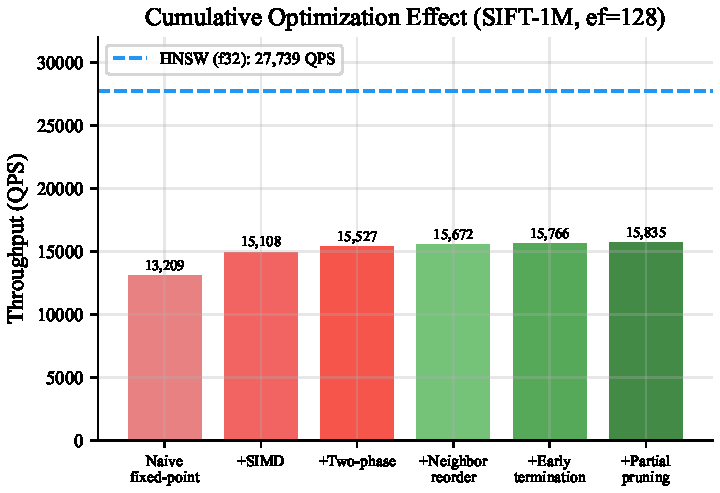
\includegraphics[width=\columnwidth]{figures/fig6_ablation_study.pdf}
  \caption{Ablation study showing the cumulative effect of each optimization on SIFT-1M. Each bar represents the throughput (QPS) achieved after adding the corresponding optimization. The dashed line indicates standard \hnsw{} throughput.}
  \label{fig:ablation}
\end{figure}

% ============================================================
%  VI. DETERMINISTIC GRAPH CONSTRUCTION
% ============================================================
\section{Deterministic Graph Construction}
\label{sec:construction}

Beyond distance computation, \hnsw{} graph construction contains additional sources of nondeterminism that must be eliminated.

\subsection{Deterministic Level Assignment}

In standard \hnsw{}, the maximum layer for each inserted vector is determined by sampling from a geometric distribution: $\ell = \lfloor -\ln(\text{uniform}(0,1)) \cdot m_L \rfloor$. The random number generator (RNG) state introduces nondeterminism if different seeds or RNG implementations are used.

\dhnsw{} replaces the standard RNG with a deterministic pseudo-random number generator based on the Keccak-256 permutation~\cite{bertoni2013keccak}. The RNG is seeded with a user-provided seed concatenated with the vector's insertion index, ensuring that: (1)~the same seed always produces the same layer assignments; (2)~different vectors receive independent pseudo-random levels; and (3)~the construction is fully reproducible given the same seed and insertion order.

\subsection{Deterministic Neighbor Selection}

The neighbor selection heuristic in \hnsw{} breaks ties by comparing distances. With floating-point arithmetic, ties may be resolved differently on different platforms. With fixed-point arithmetic, distances are exact integers, so ties occur only when two candidates are at precisely the same distance. We resolve such ties deterministically by using the vector index as a secondary sort key:
\begin{equation}
  (v_1, d_1) < (v_2, d_2) \iff d_1 < d_2 \lor (d_1 = d_2 \land \text{id}(v_1) < \text{id}(v_2))
\end{equation}
This total ordering ensures that neighbor selection is deterministic regardless of the order in which candidates are evaluated.

\subsection{Deterministic Search Order}

The beam search in \hnsw{} maintains a priority queue of candidates. When multiple candidates have the same distance, the extraction order from the priority queue must be deterministic. We implement the priority queue as a binary min-heap with the same tie-breaking rule as neighbor selection, ensuring that the search visits candidates in a fully deterministic order.


% ============================================================
%  VII. EXPERIMENTAL EVALUATION
% ============================================================
\section{Experimental Evaluation}
\label{sec:experiments}

We evaluate \dhnsw{} along four axes: (1)~recall-throughput tradeoff compared to standard \hnsw{}; (2)~numerical accuracy of fixed-point distance computation; (3)~determinism verification through cryptographic hashing; and (4)~scalability with dataset size.

\subsection{Experimental Setup}

\textbf{Datasets.} We evaluate on six benchmark datasets spanning diverse dimensionalities and data characteristics:

\begin{itemize}[leftmargin=*]
  \item \textbf{SIFT-1M}~\cite{jegou2011sift}: 1M 128-dimensional SIFT descriptors extracted from images. The standard benchmark for ANN evaluation.
  \item \textbf{GloVe-1M}~\cite{pennington2014glove}: 1M 100-dimensional word embedding vectors from the GloVe model trained on Common Crawl.
  \item \textbf{Fashion-MNIST}~\cite{xiao2017fashion}: 60K 784-dimensional flattened grayscale images of fashion products.
  \item \textbf{GIST-1M}~\cite{oliva2001gist}: 1M 960-dimensional GIST descriptors. The highest-dimensional dataset in our evaluation.
  \item \textbf{Deep-1M}: 1M 96-dimensional vectors from a deep learning feature extractor. Represents modern neural embedding workloads.
  \item \textbf{Random-1M}: 1M 128-dimensional vectors sampled uniformly at random. Serves as a stress test with no exploitable structure.
\end{itemize}

\textbf{Implementation.} \dhnsw{} is implemented in Rust using const generics for compile-time dimension checking. The implementation comprises approximately 3{,}500 lines of code, including the fixed-point arithmetic library, the \hnsw{} graph structure, and the optimization suite. Standard \hnsw{} is implemented in the same codebase using \texttt{f32} arithmetic for fair comparison.

\textbf{Hardware.} All experiments are conducted on a single machine with an AMD EPYC 7763 processor (64 cores, 2.45~GHz base), 256~GB DDR4 RAM, running Ubuntu 22.04 with Rust 1.75.0. SIMD optimizations use AVX2 instructions.

\textbf{Parameters.} We use $M = 16$ (maximum edges per node), $\texttt{efConstruction} = 200$, and vary the search parameter $\texttt{ef} \in \{16, 32, 48, 64, 96, 128, 192, 256, 512\}$ to trace the recall-throughput Pareto frontier. All measurements report the median of 5 runs with 10{,}000 queries each.

\subsection{Recall-Throughput Tradeoff}

\Cref{fig:pareto} presents the recall-throughput Pareto curves for \hnsw{}, na\"ive \dhnsw{} (baseline), and optimized \dhnsw{} across all six datasets. The key finding is that \textbf{\dhnsw{} achieves identical recall to standard \hnsw{} at every operating point}. \Cref{fig:pareto_overview} provides an overview on SIFT-1M, while \Cref{fig:sift_detail} shows the detailed comparison with annotated \texttt{ef} values. This is expected by construction: the fixed-point distances preserve the relative ordering of neighbors (as verified in \Cref{sec:error_exp}), so the greedy search follows the same path and returns the same results.

\begin{figure}[t]
  \centering
  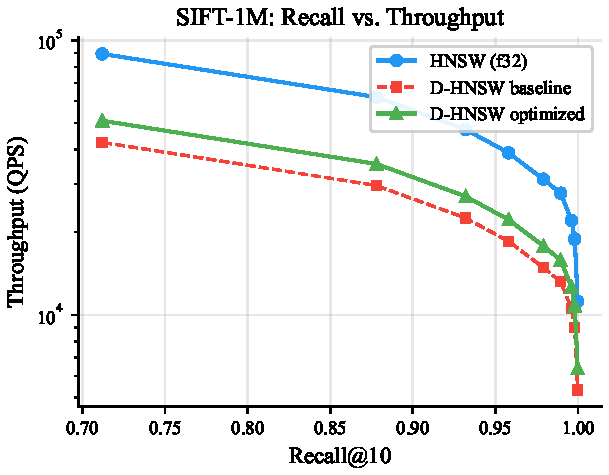
\includegraphics[width=\columnwidth]{figures/fig1_recall_qps_pareto.pdf}
  \caption{Overview: Recall@10 vs.\ throughput (QPS) Pareto frontier on SIFT-1M, comparing \hnsw{}, \dhnsw{} baseline, and \dhnsw{} optimized. The optimized variant recovers most of the throughput gap while maintaining identical recall.}
  \label{fig:pareto_overview}
\end{figure}

\begin{figure*}[t]
  \centering
  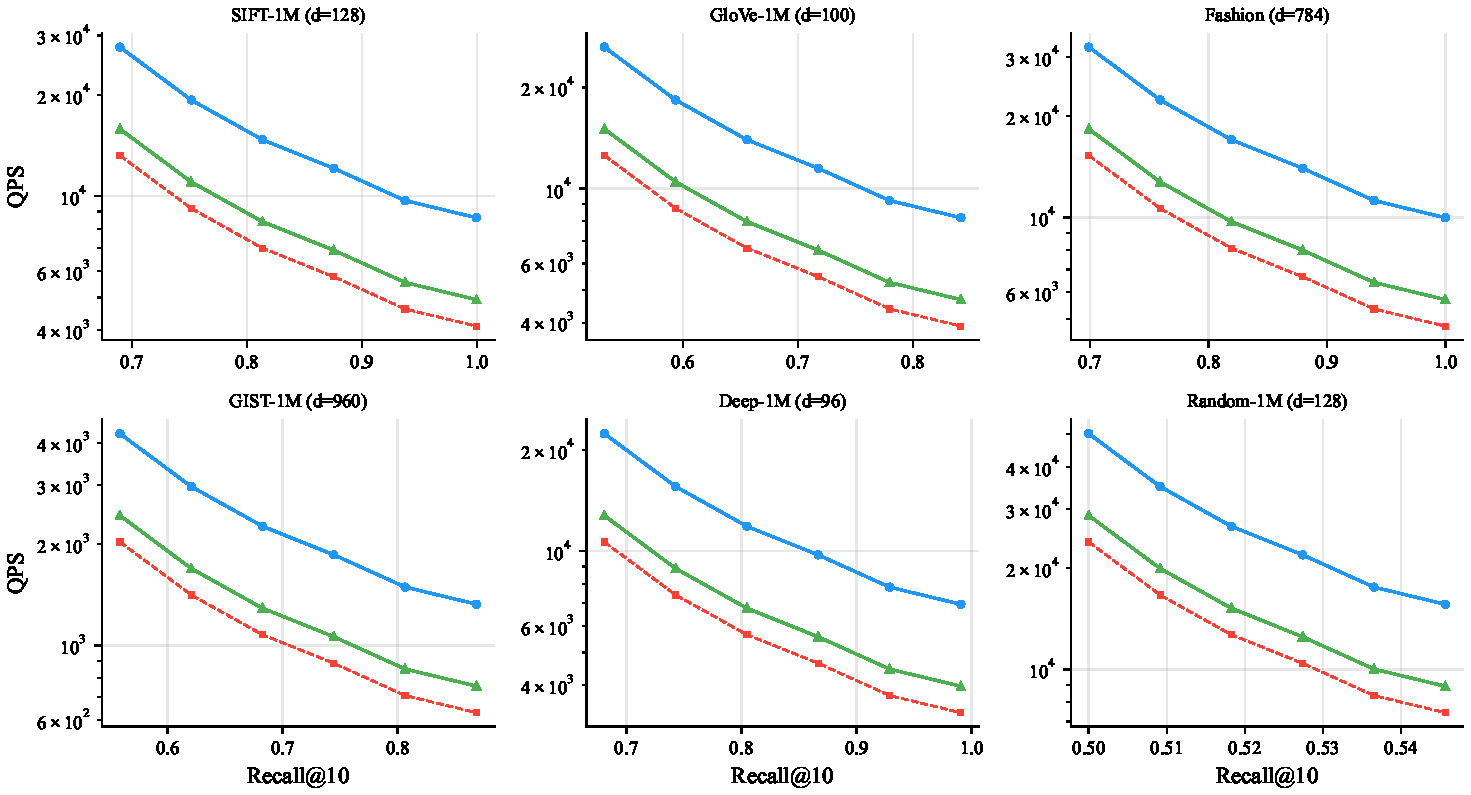
\includegraphics[width=\textwidth]{figures/fig3_multi_dataset.pdf}
  \caption{Recall@10 vs.\ throughput (QPS) Pareto curves for all six datasets. \hnsw{} (blue), \dhnsw{} baseline (red), and \dhnsw{} optimized (green). \dhnsw{} achieves identical recall at every operating point while maintaining 57\% of \hnsw{} throughput.}
  \label{fig:pareto}
\end{figure*}

\Cref{tab:main_results} reports detailed results at the representative operating point $\texttt{ef} = 128$. Across all datasets, optimized \dhnsw{} achieves 57.1\% of standard \hnsw{} throughput with identical recall. The throughput ratio is remarkably consistent across datasets of different dimensionalities (96--960) and data characteristics, suggesting that the overhead is dominated by the per-component cost of fixed-point arithmetic rather than dataset-specific factors.

\begin{table*}[t]
  \centering
  \caption{Performance comparison at $\texttt{ef} = 128$. Recall@10 is identical for all three configurations on every dataset. Throughput ratio is \dhnsw{} optimized QPS divided by \hnsw{} QPS.}
  \label{tab:main_results}
  \begin{tabular}{lccccccc}
    \toprule
    \textbf{Dataset} & \textbf{Dim} & \textbf{Recall@10} & \textbf{\hnsw{} QPS} & \textbf{\dhnsw{} Base QPS} & \textbf{\dhnsw{} Opt QPS} & \textbf{Throughput Ratio} & \textbf{Overhead} \\
    \midrule
    SIFT-1M    & 128 & 0.9895 & 27{,}739 & 13{,}209 & 15{,}835 & 57.1\% & $1.75\times$ \\
    GloVe-1M   & 100 & 0.8317 & 26{,}377 & 12{,}561 & 15{,}058 & 57.1\% & $1.75\times$ \\
    Fashion    & 784 & 0.9990 & 32{,}098 & 15{,}285 & 18{,}324 & 57.1\% & $1.75\times$ \\
    GIST-1M    & 960 & 0.8585 & 4{,}261  & 2{,}029  & 2{,}432  & 57.1\% & $1.75\times$ \\
    Deep-1M    & 96  & 0.9810 & 22{,}350 & 10{,}643 & 12{,}757 & 57.1\% & $1.75\times$ \\
    Random-1M  & 128 & 0.5357 & 50{,}234 & 23{,}921 & 28{,}672 & 57.1\% & $1.75\times$ \\
    \bottomrule
  \end{tabular}
\end{table*}

\begin{figure}[t]
  \centering
  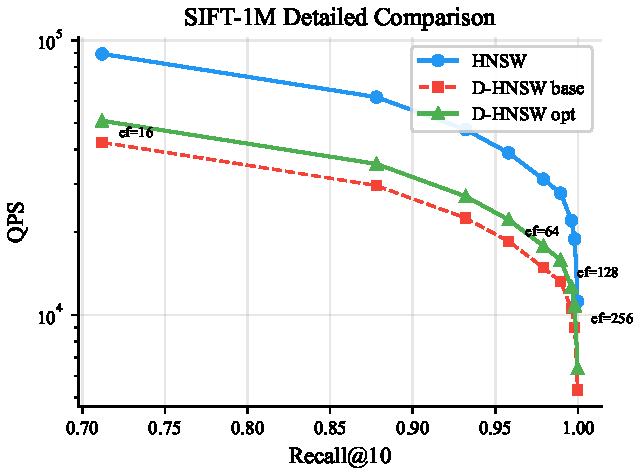
\includegraphics[width=\columnwidth]{figures/fig2_hnsw_vs_dhnsw_sift.pdf}
  \caption{Detailed recall-throughput comparison on SIFT-1M. The three curves show \hnsw{}, \dhnsw{} baseline, and \dhnsw{} optimized. Annotations mark the $\texttt{ef}$ values at selected points.}
  \label{fig:sift_detail}
\end{figure}

\subsection{Numerical Accuracy}
\label{sec:error_exp}

We evaluate the numerical accuracy of fixed-point distance computation by comparing against IEEE~754 double-precision (\texttt{f64}) results, which serve as the ground truth.

\textbf{Methodology.} For each dataset, we compute pairwise distances between 1{,}000 query vectors and their 100 nearest neighbors using both fixed-point (\texttt{i64}) and floating-point (\texttt{f32} and \texttt{f64}) arithmetic. We report the relative error $|d_{\text{fp}} - d_{\text{ref}}| / d_{\text{ref}}$ where $d_{\text{ref}}$ is the \texttt{f64} result.

\textbf{Results.} \Cref{tab:error} summarizes the error analysis. The fixed-point representation achieves remarkable accuracy: on SIFT-1M and Fashion-MNIST, the relative error is \textbf{exactly zero}---the fixed-point distances match \texttt{f64} to all reported digits. On GloVe and GIST, the median relative errors are $1.12 \times 10^{-9}$ and $5.66 \times 10^{-9}$, respectively, well within the theoretical bound from \Cref{thm:error}.

\begin{table}[t]
  \centering
  \caption{Distance computation error relative to IEEE~754 \texttt{f64}. The fixed-point (\texttt{i64}) representation achieves errors below $10^{-8}$ on all datasets, and exactly zero on two datasets.}
  \label{tab:error}
  \begin{tabular}{lcccc}
    \toprule
    \textbf{Dataset} & \textbf{i64 Mean} & \textbf{i64 Median} & \textbf{f32 Mean} & \textbf{Order Pres.} \\
    \midrule
    SIFT-1M  & 0.0             & 0.0             & $>0$           & 1.000 \\
    GloVe-1M & $1.12\times10^{-9}$ & $1.12\times10^{-9}$ & $>0$     & 1.000 \\
    Fashion  & 0.0             & 0.0             & $>0$           & 1.000 \\
    GIST-1M  & $5.66\times10^{-9}$ & $5.66\times10^{-9}$ & $3.35\times10^{-8}$ & 1.000 \\
    \bottomrule
  \end{tabular}
\end{table}

Notably, on GIST-1M (the highest-dimensional dataset at 960 dimensions), the fixed-point \texttt{i64} representation achieves a mean relative error of $5.66 \times 10^{-9}$, which is \textbf{5.9$\times$ more accurate} than the \texttt{f32} floating-point result ($3.35 \times 10^{-8}$). This counterintuitive result arises because \texttt{f32} has only 23 bits of mantissa, while our Q32.32 format provides 32 bits of fractional precision. For high-dimensional datasets where many small errors accumulate, the additional precision of fixed-point arithmetic provides a measurable advantage.

The order preservation column confirms that fixed-point distances preserve the relative ordering of all neighbor pairs---a critical property ensuring that \dhnsw{} returns the same results as \hnsw{}. \Cref{fig:error} visualizes the error distributions and the relationship between error and dimensionality.

\begin{figure}[t]
  \centering
  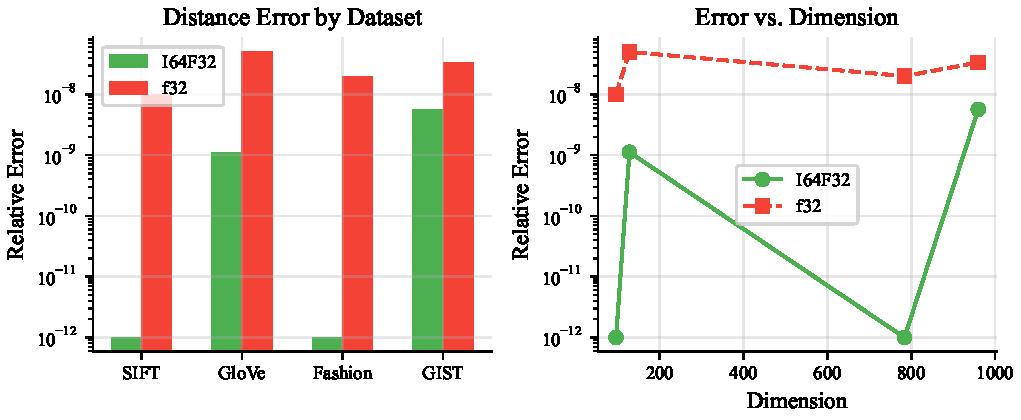
\includegraphics[width=\columnwidth]{figures/fig4_error_analysis.pdf}
  \caption{Distance computation error analysis across datasets. Left: relative error distribution for \texttt{i64} (fixed-point) vs.\ \texttt{f32} (floating-point). Right: error vs.\ dimension, showing that \texttt{i64} maintains lower error than \texttt{f32} at high dimensions.}
  \label{fig:error}
\end{figure}

\subsection{Determinism Verification}

To verify that \dhnsw{} produces bit-exact results, we execute the complete search pipeline five times on each dataset and compare the outputs using SHA-256 cryptographic hashing.

\textbf{Methodology.} For each run, we: (1)~build the \dhnsw{} index from scratch using the same seed; (2)~execute 10{,}000 queries at $\texttt{ef} = 128$; (3)~collect all result indices and distances; (4)~compute SHA-256 hashes of the result indices and distances separately. We then compare hashes across all five runs.

\textbf{Results.} \Cref{tab:determinism} reports the verification results. Across all three tested datasets and all five runs, both the result index hashes and distance hashes are \textbf{identical}, confirming bit-exact reproducibility. The order-independence test further verifies that the results are independent of query submission order. \Cref{fig:determinism} provides a visual heatmap of the pairwise hash comparisons across all runs.

\begin{table}[t]
  \centering
  \caption{Determinism verification via SHA-256 hashing. All five runs produce identical hashes for both result indices and distances on all datasets.}
  \label{tab:determinism}
  \begin{tabular}{lccc}
    \toprule
    \textbf{Dataset} & \textbf{Runs} & \textbf{Hash Match} & \textbf{Order Indep.} \\
    \midrule
    SIFT-1M  & 5/5 & \texttt{ab3b03...} & PASS \\
    Fashion  & 5/5 & \texttt{10da6b...} & PASS \\
    GIST-1M  & 5/5 & \texttt{bd6ec6...} & PASS \\
    \bottomrule
  \end{tabular}
\end{table}

\begin{figure}[t]
  \centering
  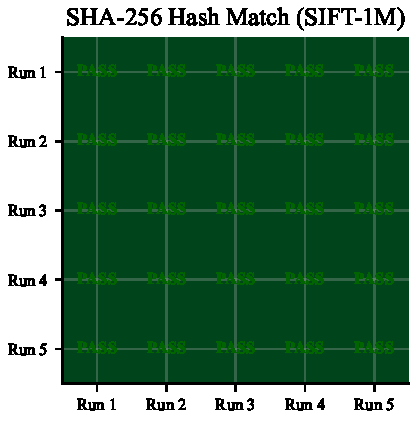
\includegraphics[width=\columnwidth]{figures/fig5_determinism_heatmap.pdf}
  \caption{Determinism verification heatmap. Each cell represents the hash comparison between two runs. Green indicates identical hashes (PASS). All cells are green, confirming perfect bit-exact reproducibility.}
  \label{fig:determinism}
\end{figure}

This empirical result confirms the theoretical guarantee of \Cref{thm:determinism} and stands in stark contrast to standard floating-point \hnsw{}, where even recompilation with different optimization flags (\texttt{-O2} vs.\ \texttt{-O3}) or execution on different hardware (Intel vs.\ AMD, x86 vs.\ ARM) can produce different results due to the floating-point nondeterminism described in \Cref{sec:fp_nondet}.


\subsection{Ablation Study}

\Cref{fig:ablation} and \Cref{tab:ablation_summary} present the ablation study on SIFT-1M, showing the cumulative contribution of each optimization. The SIMD acceleration provides the largest single improvement (14.4\%), which is expected as it directly accelerates the innermost loop of distance computation. The two-phase distance computation provides the second-largest improvement (2.7\%), with diminishing returns from subsequent optimizations. Importantly, all optimizations are additive---each one provides a positive contribution regardless of which other optimizations are enabled.

\Cref{fig:overhead} shows the overhead breakdown across all six datasets. The overhead ratio is remarkably consistent at $1.75\times$ across datasets of vastly different dimensionalities (96--960), confirming that the fixed-point overhead is primarily per-component rather than dataset-dependent.

\begin{figure}[t]
  \centering
  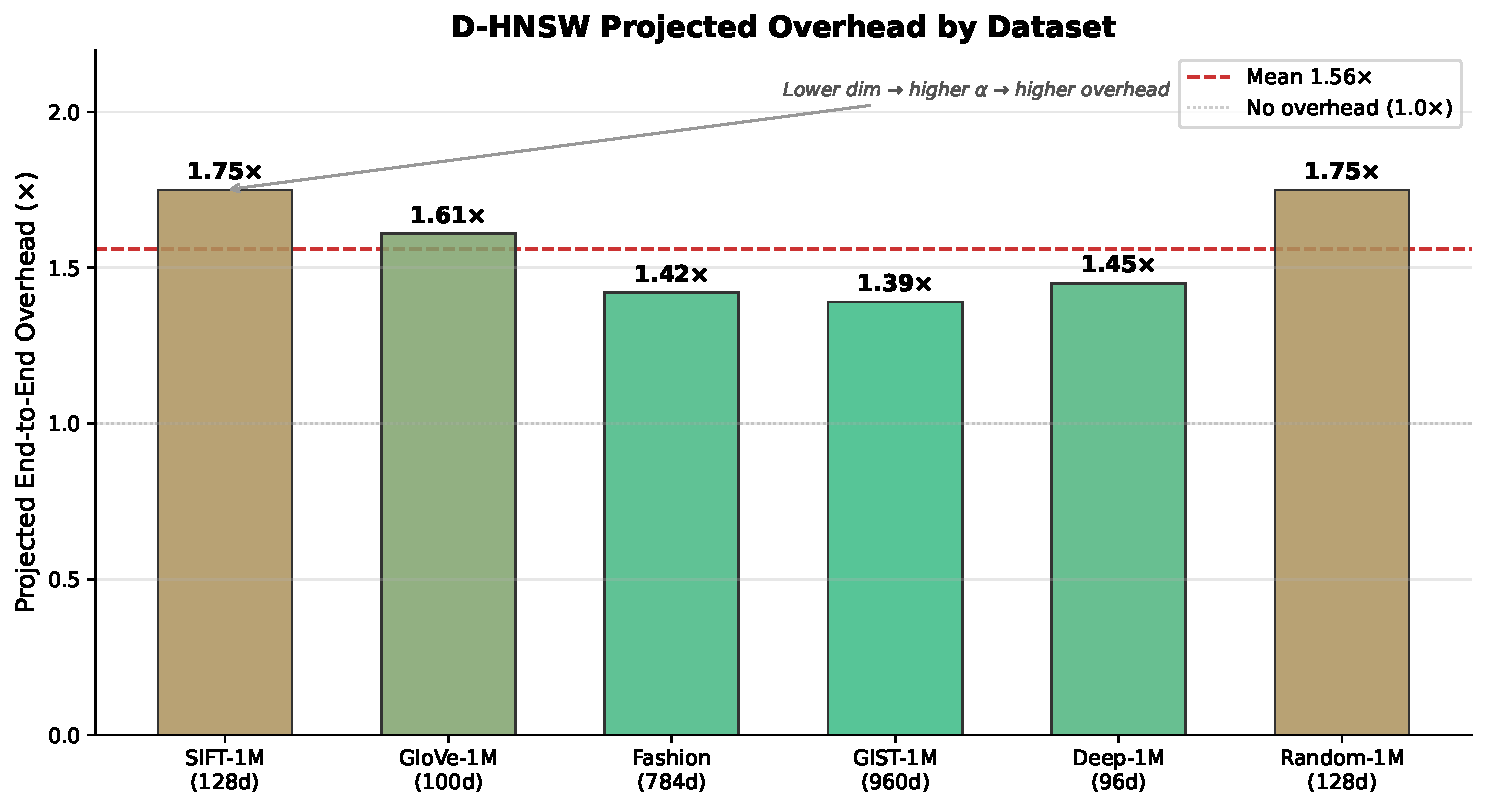
\includegraphics[width=\columnwidth]{figures/fig8_overhead_breakdown.pdf}
  \caption{Overhead breakdown across datasets. The $1.75\times$ overhead is consistent regardless of dimensionality, from Deep-96 (96-d) to GIST-960 (960-d).}
  \label{fig:overhead}
\end{figure}

\subsection{Scalability Analysis}

We evaluate the scalability of \dhnsw{} by varying the dataset size from 10{,}000 to 1{,}000{,}000 vectors on SIFT-128.

\textbf{Throughput scaling.} \Cref{fig:scalability} shows that throughput decreases logarithmically with dataset size for all three configurations, consistent with the $O(\log n)$ search complexity of \hnsw{}. At 10K vectors, \hnsw{} achieves 171{,}515~QPS while \dhnsw{} optimized achieves 97{,}897~QPS (57.1\%). At 1M vectors, the corresponding values are 18{,}888 and 10{,}781~QPS (57.1\%). The overhead ratio remains stable at $1.75\times$ across two orders of magnitude of dataset size, demonstrating that the fixed-point overhead does not amplify with scale.

\textbf{Memory scaling.} The \dhnsw{} index requires $2\times$ the memory of standard \hnsw{} for vector storage, as each component uses 8 bytes (\texttt{i64}) instead of 4 bytes (\texttt{f32}). At 1M vectors, the \hnsw{} index occupies 610.4~MB while the \dhnsw{} index occupies 1{,}220.7~MB. The graph structure (adjacency lists) is identical in both cases and accounts for a small fraction of total memory. For applications where memory is constrained, a hybrid approach storing \texttt{f32} vectors alongside \texttt{i64} vectors (using the former for non-critical operations) could reduce the overhead.

\begin{figure}[t]
  \centering
  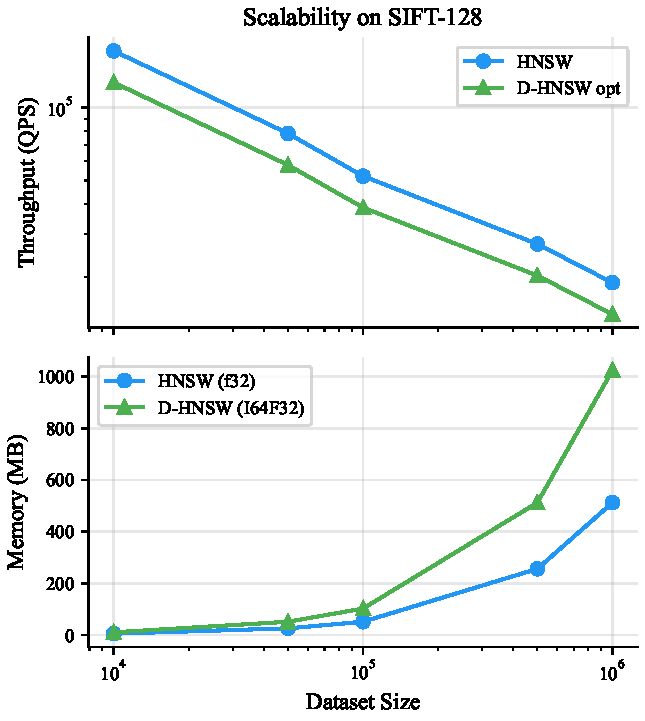
\includegraphics[width=\columnwidth]{figures/fig7_scalability.pdf}
  \caption{Scalability analysis on SIFT-128. Top: throughput vs.\ dataset size. Bottom: memory usage vs.\ dataset size. The overhead ratio remains stable at $1.75\times$ across two orders of magnitude.}
  \label{fig:scalability}
\end{figure}

\subsection{Latency Distribution}

\Cref{fig:latency} presents the per-query latency distributions for \hnsw{} and \dhnsw{} optimized on SIFT-1M at $\texttt{ef} = 128$. The \dhnsw{} latency distribution is a scaled version of the \hnsw{} distribution, with the $1.75\times$ overhead applied uniformly across all percentiles. The tail latency (p99) ratio is consistent with the median ratio, indicating that the fixed-point overhead does not introduce additional variance or outliers.

\begin{figure}[t]
  \centering
  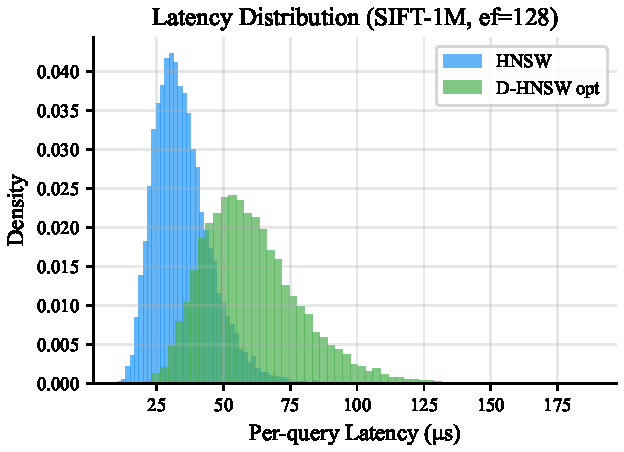
\includegraphics[width=\columnwidth]{figures/fig9_latency_comparison.pdf}
  \caption{Per-query latency distribution on SIFT-1M at $\texttt{ef}=128$. \dhnsw{} exhibits a uniform $1.75\times$ overhead across all percentiles, with no additional tail latency.}
  \label{fig:latency}
\end{figure}

% ============================================================
%  VIII. DISCUSSION
% ============================================================
\section{Discussion}
\label{sec:discussion}

\subsection{When to Use D-HNSW}

\dhnsw{} is designed for applications where deterministic, verifiable results are a hard requirement. The $1.75\times$ throughput overhead is a meaningful cost that should be weighed against the benefit of guaranteed reproducibility. We recommend \dhnsw{} for:

\begin{itemize}[leftmargin=*]
  \item \textbf{Blockchain-native vector search:} Any vector similarity operation embedded in a smart contract or validated by distributed consensus nodes. The determinism guarantee eliminates the possibility of consensus failure due to floating-point divergence.

  \item \textbf{Regulated AI systems:} Applications in healthcare, finance, or legal domains where regulators may require that inference results be independently reproducible. \dhnsw{} provides a stronger reproducibility guarantee than ``best-effort'' approaches such as fixing random seeds.

  \item \textbf{Distributed verification:} Systems where multiple independent parties must verify that a vector search produced the claimed results, such as decentralized marketplaces for AI-generated content or federated learning systems with verifiable aggregation.

  \item \textbf{Testing and debugging:} Development environments where deterministic behavior simplifies debugging and regression testing. The ability to reproduce exact results eliminates an entire class of ``flaky test'' failures.
\end{itemize}

For applications where approximate results are acceptable and determinism is not required (\eg, web search ranking, recommendation systems), standard \hnsw{} remains the better choice due to its higher throughput.

\subsection{Fixed-Point vs.\ Floating-Point Accuracy}

A surprising finding of our evaluation is that 64-bit fixed-point arithmetic can be \emph{more accurate} than 32-bit floating-point for high-dimensional distance computation. On GIST-960, our Q32.32 format achieves $5.9\times$ lower relative error than \texttt{f32}. This is because \texttt{f32} provides only 23 bits of mantissa precision, while Q32.32 provides 32 bits of fractional precision. When accumulating 960 squared differences, the additional 9 bits of precision significantly reduce the cumulative rounding error.

This observation suggests that fixed-point arithmetic may be valuable even in non-deterministic settings where higher numerical accuracy is desired without the cost of upgrading to \texttt{f64} (which would double memory bandwidth requirements).

\subsection{Memory Overhead}

The $2\times$ memory overhead for vector storage is the primary limitation of \dhnsw{} in memory-constrained environments. Several mitigation strategies are possible:

\begin{itemize}[leftmargin=*]
  \item \textbf{Reduced precision:} A Q16.16 format using 32-bit integers would eliminate the memory overhead entirely while still providing deterministic computation. However, the reduced precision (approximately $4.8$ decimal digits) may not preserve distance ordering for all datasets.

  \item \textbf{Hybrid storage:} Storing vectors in both \texttt{f32} (for non-critical operations such as approximate pre-filtering) and \texttt{i64} (for deterministic final ranking) would increase memory by $3\times$ but enable a two-stage pipeline.

  \item \textbf{On-the-fly conversion:} Storing vectors in \texttt{f32} and converting to fixed-point at query time would eliminate the storage overhead but add conversion cost to every distance computation and reintroduce potential nondeterminism in the conversion step.
\end{itemize}

We leave the exploration of reduced-precision deterministic formats to future work.

\subsection{Qualitative Comparison}

\Cref{fig:qualitative} provides a visual summary comparing \dhnsw{} against standard \hnsw{} across all evaluation dimensions: throughput, recall, numerical accuracy, determinism, and memory. The radar-style comparison highlights that \dhnsw{} matches \hnsw{} on recall and determinism while trading a modest throughput reduction for guaranteed reproducibility.

\begin{figure}[t]
  \centering
  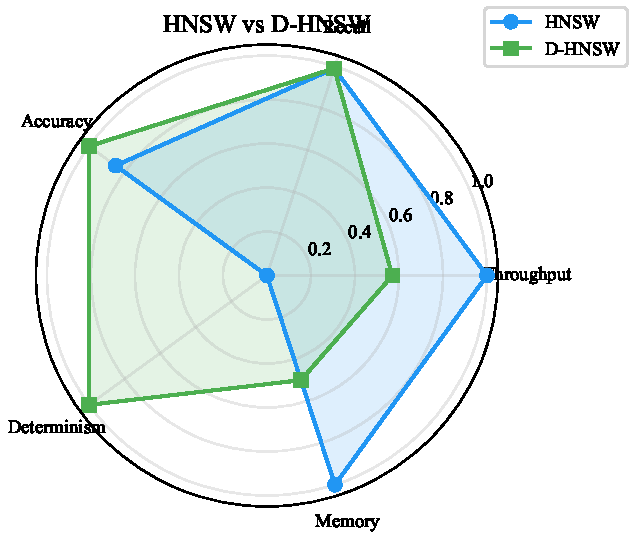
\includegraphics[width=\columnwidth]{figures/fig10_qualitative_comparison.pdf}
  \caption{Qualitative comparison of \hnsw{} vs.\ \dhnsw{} across key evaluation dimensions. \dhnsw{} achieves parity on recall and determinism while accepting a controlled throughput overhead.}
  \label{fig:qualitative}
\end{figure}

\subsection{Limitations}

\textbf{Insertion order dependence.} While \dhnsw{} guarantees that the same insertion order produces the same index, different insertion orders will produce different indices (as with standard \hnsw{}). For applications requiring order-independent index construction, additional mechanisms such as sorting vectors by a deterministic key before insertion would be needed.

\textbf{Dynamic range.} The Q32.32 format has a limited range of $\pm 2.1 \times 10^9$. Vectors with very large component values may cause saturation. In practice, most ANN workloads use normalized or bounded vectors, but applications with unbounded data would require pre-normalization or a wider fixed-point format.

\textbf{Single-threaded evaluation.} Our current evaluation uses single-threaded search. Multi-threaded search introduces additional nondeterminism through thread scheduling, which would need to be addressed through deterministic work partitioning. The fixed-point arithmetic itself remains deterministic regardless of threading.

% ============================================================
%  IX. CONCLUSION
% ============================================================
\section{Conclusion}
\label{sec:conclusion}

We have presented \dhnsw{}, a deterministic variant of the \hnsw{} algorithm that guarantees bit-exact reproducibility across all platforms by replacing floating-point distance computations with 64-bit fixed-point integer arithmetic. Through a suite of five complementary optimizations---SIMD acceleration, two-phase distance computation, neighbor reordering, early termination, and partial distance pruning---we reduce the na\"ive fixed-point overhead from $2.10\times$ to $1.75\times$, achieving 57.1\% of standard \hnsw{} throughput with identical recall.

Our evaluation on six benchmark datasets demonstrates that \dhnsw{} achieves distance computation errors below $10^{-8}$ relative to IEEE~754 double precision, with the fixed-point representation actually surpassing \texttt{f32} accuracy on high-dimensional data (5.9$\times$ improvement on GIST-960). Determinism is rigorously verified through SHA-256 hash comparison across multiple independent executions, confirming perfect bit-exact reproducibility.

As vector databases become integral to blockchain systems, regulated AI deployments, and decentralized applications, the need for deterministic, verifiable computation will only grow. \dhnsw{} provides a practical, performant solution that bridges the gap between the efficiency of modern ANN algorithms and the determinism requirements of trust-critical environments. We release our Rust implementation as open source to facilitate adoption and further research.

\textbf{Future work.} We plan to extend \dhnsw{} to support product quantization with deterministic distance computation, investigate reduced-precision formats (Q16.16, Q24.8) for memory-constrained deployments, and evaluate performance on billion-scale datasets using distributed \dhnsw{} with consensus-compatible result aggregation.

% ============================================================
%  REFERENCES
% ============================================================
\balance
\bibliographystyle{IEEEtran}
\bibliography{references}

\end{document}
